\subsection{Beyond ``embarrassignly parallel''}
\makesubcontentsslidessec

\begin{frame}
  \begin{block}{A brief personal history of parallel computing}
  \includegraphics[width=\textwidth]{../common/pics/hardware/ParallelHardware28.pdf}
  \end{block}
\end{frame}

\begin{frame}{Early Work in Statistics: Crossproduct (Row-Block layout)}
  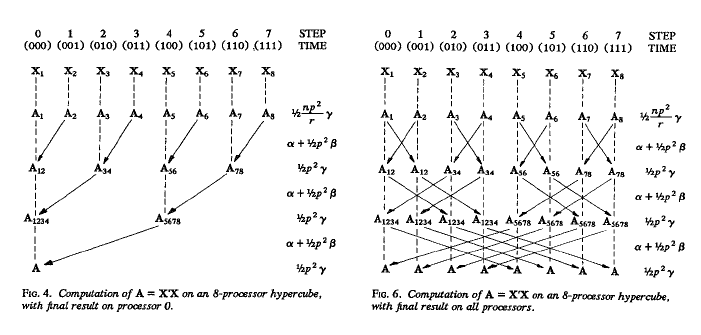
\includegraphics[width=\textwidth]
  {../common/pics/comm/Crossprod1987.png} \\
  \begin{block} {\scriptsize Ostrouchov (1987). Parallel Computing on a
      Hypercube: An overview of the architecture and some
      applications. {\em Proceedings of the 19th Symposium on the
        Interface of Computer Science and Statistics}, p.27-32.}
  \end{block}
\end{frame}

\begin{frame}{Distributed Numerical Linar Algebra}
  \begin{block}{BLACS Library Communication Patterns (ScaLAPACK)}
    \begin{minipage}{1.8cm}\vspace{-1cm}
      
\includegraphics[width=2cm]{../common/pics/comm/BLACS01.png} \\[-1ex]
      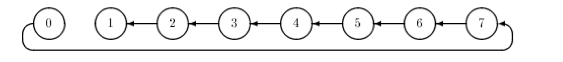
\includegraphics[width=2cm]{../common/pics/comm/BLACS02.png} \\[-1ex]
      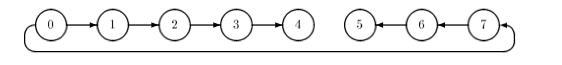
\includegraphics[width=2cm]{../common/pics/comm/BLACS03.png} \\[-.3ex]
      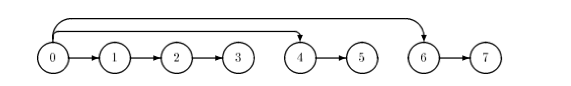
\includegraphics[width=2cm]{../common/pics/comm/BLACS04.png}
    \end{minipage}
    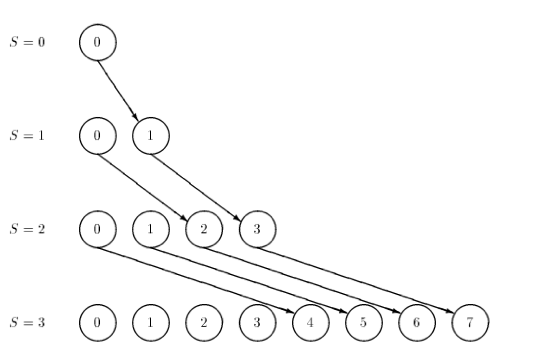
\includegraphics[width=2cm]{../common/pics/comm/BLACS05.png}
    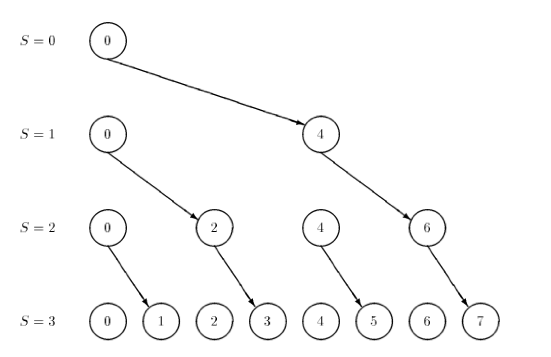
\includegraphics[width=2cm]{../common/pics/comm/BLACS06.png}
    \begin{minipage}{1.8cm}\vspace{-.5cm}
      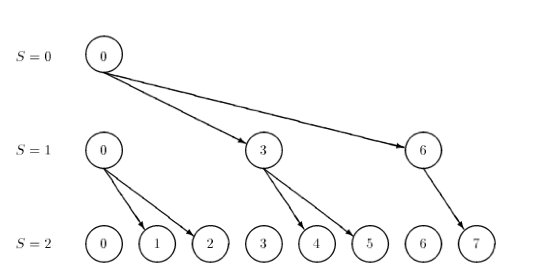
\includegraphics[width=2cm]{../common/pics/comm/BLACS07.png} \\
      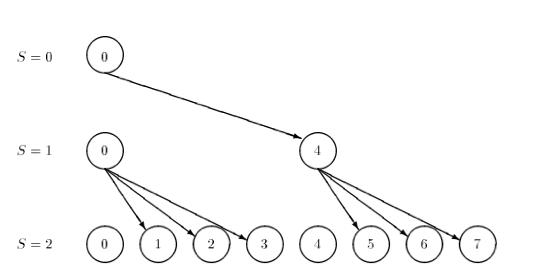
\includegraphics[width=2cm]{../common/pics/comm/BLACS08.png}
    \end{minipage}
    \begin{minipage}{1.9cm}\vspace{-.1cm}
      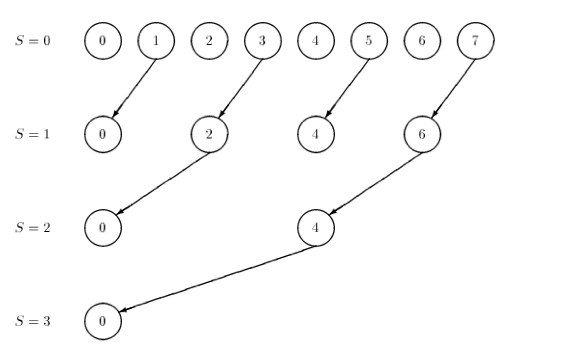
\includegraphics[width=2cm]{../common/pics/comm/BLACS09.png} \\
      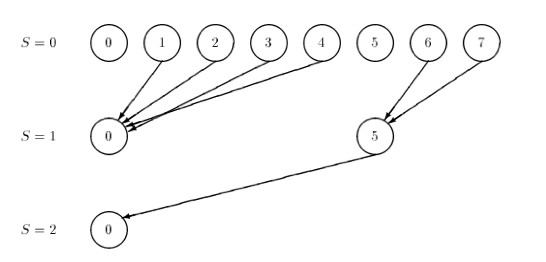
\includegraphics[width=2cm]{../common/pics/comm/BLACS10.png}
    \end{minipage}
    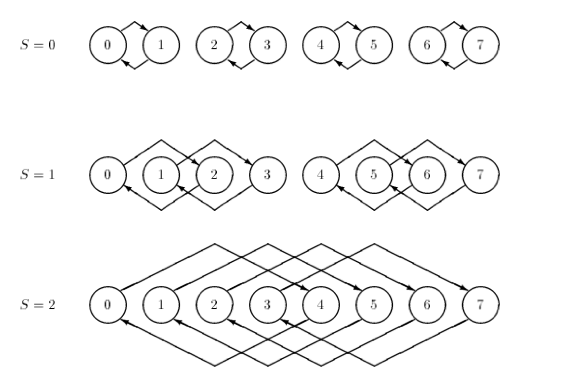
\includegraphics[width=1.9cm]{../common/pics/comm/BLACS11.png}
  \end{block}
  \begin{block}{\scriptsize J. Dongarra and R. C. Whaley (1995). A
      User’s Guide to the BLACS v1.1. {\em UT-CS-95-281}, March 1995.}
    \begin{itemize}
    \item Complex communications for block-distributed numerical
      linear algebra computations.
    \item Enables use of separate rowwise and columnwise
      communicators.
    \item Optimizes collective operations of multiple communicators.
    \end{itemize}
  \end{block}
\end{frame}

% \begin{frame}
%   \begin{block}{Communication complexity: Block Data layout dependence}
%     \begin{center}
%      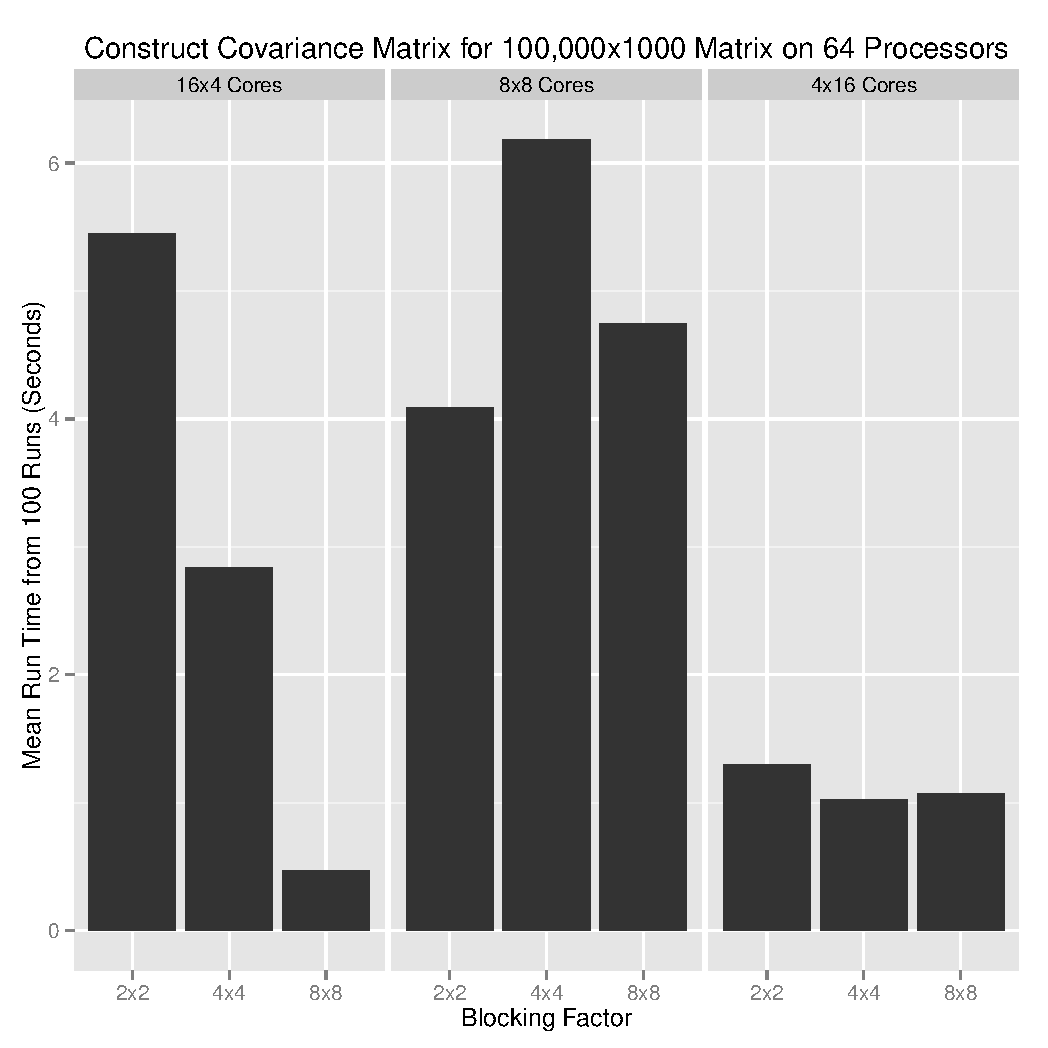
\includegraphics[width=10cm, height=7cm]{../common/pics/cov_param}
%     \end{center}
%   \end{block}
% \end{frame}

\begin{frame}{PaRSEC: Parallel Runtime Scheduling and Execution
    Controller (DPLASMA)}
  \vspace{-.1cm}
  \hspace{2cm}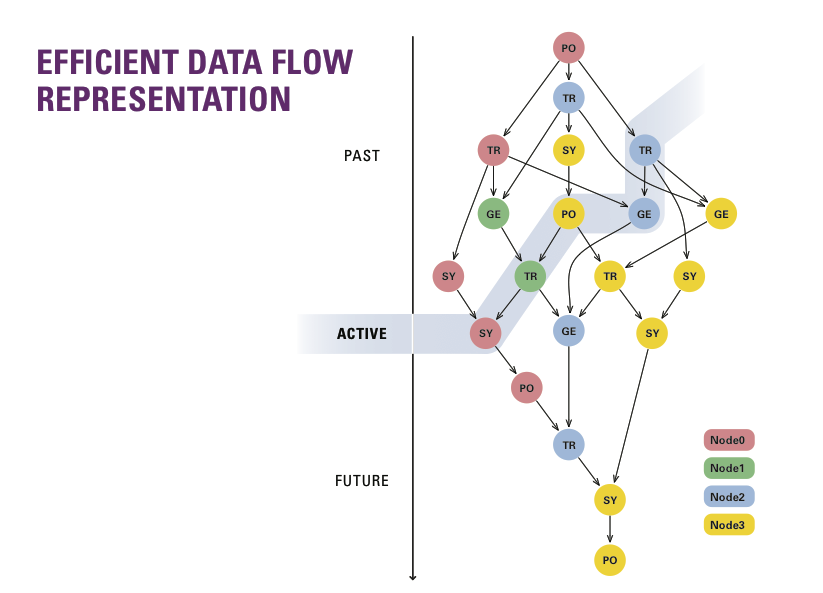
\includegraphics[trim=0cm 0cm 0cm
  1cm,clip=true,width=7.5cm]{../common/pics/comm/PaRSEC1.png}
 \\[-3.4cm]
  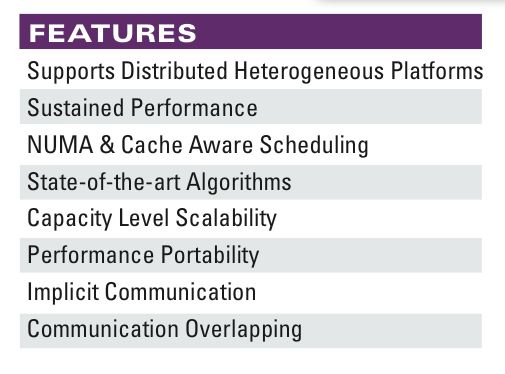
\includegraphics[width=4cm]{../common/pics/comm/PaRSEC2.png}
  \hspace{5cm}{\tiny Graphic from icl.cs.utk.edu}
  \begin{block}
    {\tiny Bosilca, G., Bouteiller, A., Danalis, A., Faverge,
      M., Herault, T., Dongarra, J. "PaRSEC: Exploiting Heterogeneity
      to Enhance Scalability," IEEE Computing in Science and
      Engineering, Vol. 15, No. 6, 36-45, November, 2013.}
    \begin{itemize}
    \item Master data flow controller runs distributed on all cores.
    \item Dynamic generation of current level in flow graph
    \item Effectively removes collective synchronizations
    \end{itemize}
  \end{block}
\end{frame}
